\documentclass{article}
\usepackage{graphicx} %package to manage images
\graphicspath{ {graphs/} }
\title{Constraint Programming and AI for Soccer Analysis}
\author{Jack Wall}
\usepackage{amsmath}
\newcommand{\vect}[1]{\boldsymbol{#1}}


\begin{document}
	
	\maketitle
	\(Abstract:\) Soccer is one of the most popular sports in the world with an estimated 265 million players actively involved, and countless more fans interested in the sport. These fans usually pose interesting questions throughout the competitions. One interesting question often asked relates to the \(qualification\ problem\) in which at some stage of the competition, if a team \(i\) still has a theoretic chance of finishing first in a league, or being the top \(n\) teams at the end of the competition. Other interesting problems in soccer would be \(the\ elimination\ problem\), \(possible\ qualification\ problem\), and \(guaranteed\ qualification\ problem\). These problems are NP-Complete when played according to the FIFA pointing rule system (3 points for a win, 1 for a draw, 0 for a loss). In this paper, we investigate the efficiency of such algorithms and attempt to predict the runtimes for such problems, in order to reduce the computational cost of solving such problems. The benefits of such predictions could be useful to fans who bet on leagues, and seek to utilise cloud computing to solve similar NP-complete problems. 
	
	\section{Introduction}
	\paragraph{}
	Soccer, or football, is the most popular sport in the world. Played by two teams, the sport has eleven players on each team. Both teams aim to score in the opposing net, while trying to minimize the number of goals made by the opposition onto their own net. These games are then grouped into a scheduled competition known as a league. Leagues are a series of games played by a fixed amount of teams.
	Each team plays every other team in a pre-defined format. Usually a single, or double round-robin schedule. The result of the game awards points to the teams in accordance with FIFA’s``Three points for a win'' method. The winning team receives 3 points, and the losing team 0. In the event of a draw, both teams are awarded 1 point each. This places more emphasis on winning a few games, rather than drawing more.


	The interesting aspect of soccer leagues, is often the top ranking teams at the end of the competition can qualify for another competition, involving better teams. This keeps the competitive spirit of teams out of contention for winning the league, as they still are eligible to finish in the top number of positions, and hence can qualify for a more prestigious competition.
	With the development of sport statistics being widely available, soccer fans have become more and more interested in the statistical information of their club. Knowing the most optimal outcome of the club standings while still being realistic can tailor the fan expectations for the club. As a result, there is great demand for software systems to aid fans to pursue such queries in a timely fashion.
	
	
	Common soccer computational problems have been studied before (e.g. the elimination problem, possible qualification problem, etc.) such as SABIO \\(http://www.sabiofutbol.com/), and the paper ``CP and MIP Approaches for Soccer Analysis''. SABIO is a football analysis website that utilises Constraint Programming principles to answer soccer related queries for fans. The paper ``CP and MIP Approaches for Soccer Analysis'' improves on SABIO, by investigating the most optimal Constraint Programming (CP) and Mixed Integer Programming (MIP) techniques to answer such problems. 
	In this paper, we will measure our own constraint programming models on various different soccer queries, drawing information and insight into the problems. We will then investigate using machine learning models to predict runtimes of the algorithms, as well as the results of some of the problems. These programs may have real world use cases that also will be examined.
	
	\newpage
	\section{Analysis}
	
	\subsection{Background Material}
	
	\subsubsection{Qualification and Elimination Problem}
	Soccer competitions offer an excellent opportunity to propose interesting problems. In this paper, we are going to investigate two of these problems. Similar problems however, have been researched in the past.
	
	\(Promotion\ and\ Relegation\): In soccer, there are often too many teams in an area to fit into one league. Instead, these teams are grouped into multiple leagues, with each team belonging to at most one league. Each league aims to contain teams of similar ability. The best teams belong to the first league, and the worst to the last league. In order to facilitate movement of teams between leagues, promotions and relegations are used. If a team finishes in the top a positions, they will be promoted to a higher quality league. However, if a team finishes in the bottom a positions, they are forced to relegate to a lesser quality league. As a result, soccer fans are eager to find out the possibility of their team being promoted or relegated, based on the remaining games in the league. Kern and Paulusma [24] also proved NP-Completeness for questions like “is there a chance that team i ends up with the lowest final score?” or “is there a chance that team i ends up being one of the three teams that have the three lowest final scores?”, which might cause a direct relegation to a lower division. They used a version of the elimination problem to prove NP-Completeness for the rule (α = 0, β = 1, γ = 3) applied in soccer.
	
	\(The\ Elimination\ Number\): The elimination number is defined as the minimum number of points that a team must get in order to have a chance of finishing in first place or to secure a place in the playoffs. Gusfield and Martel [20] showed that computing such number of points for soccer is NP-Hard and this problem is at least as hard as solving the subset sum problem [23].
	
	\(Guaranteed\ Qualification\ Problem\): This problem as defined in [37] consists of “calculating the minimum number of points any team has to win in order to be qualified, regardless of any other results”. It was tackled by Riberio et al. [27, 37] using integer programming. They calculated a guaranteed qualification score (GQS) and their implementation can also be used to determine if a team is mathematically qualified to the playoffs. Later in 2014, Raack et al. [33] develop a general integer programming model for rankings to calculate the number of points needed to guarantee a team the ith place. The model proposed is very general and can be applied to many sports that use a league based format.
	
	\(Possible\ Qualification\ Problem\): This problem defined in [37] can be defined as “computing how many points each team has to win to have any chance to be qualified”. Riberio et al. [27, 37] studied this problem using integer programming for which they calculated a possible qualification score (PQS). This score depends on the current standings of every team in the table, and the remaining games within the league. This model can be used to check if a team is mathematically eliminated from the playoffs, if their current number of points plus the total number of possible points (i.e. if they win their remaining games) is less than it's PQS. 
	In soccer, the scheduling problem has been studied in many different tournaments and leagues. For example, Noronha et al. [31] proposed an integer programming formulation and a branch-and-cut strategy to schedule a highly constrained Chilean soccer tournament. Related approaches include scheduling for the Belgian soccer league [17], a triple round robin tournament for the Danish soccer league [34] and the professional soccer leagues of Austria and Germany [3]
	
	\(Minimum\ Number\ of\ Losses\ Problem:\) In this paper, one of the main problems we will be investigating, is the minimum number of losses problem. At a particular stage of the competition, a given team may want to set realistic goals for the end of the league e.g. finish in position \(x\), win the \(y\) remaining games, etc.. One approach to these problems is to phrase them as a minimum number of losses problem. ``What is the minimum number of losses team a can encounter, while still finishing in position \(x\)''. This problem is a variation of the \(Guaranteed\ Qualification\ Problem\), with the difference being the addition of minimising the number of losses. This significantly increases the complexity of the problem, as instead of looking for the first solution, we search for the optimal solution, according to the number of losses.
	
	
	
	
	\subsubsection{Elimination Problem Complexity}
	The desired solution to the elimination problem can be defined as “determining for a given team whether or not they are already eliminated, i.e., whether or not they can no longer become champions” \cite{threepointrule}. Any team i can be defined as eliminated if team i wins the remaining games in the league, there will still be at least one team in a position better than i. The complexity of this problem depends on the way how scores are allocated according to the outcome of every match \cite{fifarules}. Kern and Paulusma \cite{fifarules} \cite{eliminationproblem} and Bernholt et al\cite{threepointrule} independently proved that for the actual pointing rule (0, 1, 3) the problem
	is NP-complete.
	
	\subsubsection{Constraint Satisfaction Problems}
	The queries that this project aims to answer are known as CSPs. Constraint Satisfaction Problems (CSPs) are a group of mathematical problems that satisfy under declared limitations or constraints. The CSP contains a set of variables, a set of domain values for the variables, and a set of constraints that must be satisfied. Each domain contains possible values for one variable. The goal is to find the domain values that satisfy every predefined constraint in order to be declared as a solution. CSPs tend to have a high complexity, due to the amount of optional solutions, in comparison with satisfiable ones. 
	In this project, the CSP will contain a finite amount of domain values, which allows us to perform a search for the solution. There are many options to choose from e.g. Linear programming, or local search. The solution in this document will use a combination of Constraint Propagation and Backtrack Search.
	
	\subsubsection{Constraint Propagation (CP)}
	Constraint Propagation is the reduction of domain sizes of each variable in a CSP, to achieve a faster computation time. It seeks to eliminate redundant values for each variable, as they will be impossible to satisfy. CP changes the problem, without altering the solution. It can also be used as an unsatisfiability checker, to see if constraints contradict, resulting in an unsatisfiable solution.
	For example, given variables \(a = [1..5]\) and \(b = [3..10]\), and constraint \(a < b\):
	Constraint Propagation will reduce the set a to values \(a = [1..2]\).
	
	\subsubsection{Backtrack Search}
	Backtrack search is an algorithm that attempts to find all possible solutions that satisfy a CSP. This search systematically and recursively checks if each value in a domain will satisfy the constraints. If a value in a domain is found to not be a part of the solution, it is discarded and the algorithm ‘backtracks’ to another value in the domain. This is repeated until all values in each domain are checked. Because Constraint Propagation can reduce the domain size, it is useful to use it in conjunction with backtrack search, as it will reduce the number of checks before a backtrack, greatly increasing the efficiency of the algorithm.
	
	\subsubsection{Search heuristics in Constraint Programming}
	% search algorithm does not need to be systematic
	A search algorithm (e.g. backtracking search) may systematically choose which variables to look at for a viable solution. Experiments of several researchers\cite{cp} have shown that the method in which values are chosen on backtracking, can significantly affect the complexity of the algorithm. There are two types of ordering: Static and dynamic. Static Ordering declares the order of values before the search begins. This contrasts with Dynamic Ordering, which declares each value at time of assignment, depending on the state of the search. Many heuristics have been developed in Constraint Programming. One of which being the “first-fail” principle. This is a variable based heuristic and is best described as follows: 
	“To succeed, try first where you are most likely to fail.”
	This method selects the variables with fewest possible alternatives. The reasoning behind “first-fail” is that the more values there are, the more likely the variable is to contain a solution. It also assumes that each value is equally likely to become a solution. This heuristic aims to reduce the depth of the search tree by encountering an early failure.
	
	
	Once a variable is chosen, there lies the choice of value within said variable. Again, there are many choices of heuristic available, as the order of values have a significant impact on the complexity of the search algorithm, unless there is no possible solution. If there is no solution, then the method of variable selection is useless. However, if there contains at least one solution, then selecting a variable based on passed instantiations would lead to an informed choice for a possible result. So we apply the “succeed-first” principle. One possible heuristic, would be to choose the value that leads to an easiest to solve CSP. This requires an estimator for the difficulty of a CSP, which can be costly. In randomly generated problems, there is not enough information to provide an educated estimate on a value likely to succeed, but with particular problems, there may be some content that can be used to improve the likeliness that such a value will succeed.
	
	
	\newpage
	\section{Design}
	\subsection{Formula}
	In this section, we describe our Constraint Programming formulation for soccer competitions. Specifically differentiating between notations, variables and constraints.
	Basic Formulation: 
	\begin{itemize}
		\item \textit{n:} number of teams in the competition;
		\item \textit{T:} set of team indexes in the competition;
		\item \textit{i, j:} team indexes such that (\(i, j \in T\))
		\item \(initialPts_i\): initial poinst of team \(i\)). If \(i\) has not played any games, then \(initialPts_i=0\);
		\item \(F\): number of fixtures left to be played in the competition. A fixture consists
		of one or more games between competitors;
		\item \(k\): represents a fixture number (\(1 \leq k \leq F\));
		\item \(G\): set that represents the schedule of the remaining games to be played. Every game is represented as a triple \(ng_e = (i,j,k)\) where k is the fixture when both teams meet in a game and \(1 \leq e \leq \mid G\mid \) if \(\mid G \mid \geq 1 \);
		\item \(gamePts_{ik}\): represents the points that team \(i\) get in fixture \(k\), (\((1 \leq k \leq F)\) and \(gamePts_{ik} \in \{ 0, 1, 3 \} \)). If team \(i\) is not scheduled to play fixture \(k\), then \(gamePts_{ik} = 0\);
		\item \(losses_{ik}\): represents whether or not team \(i\) encountered a loss at fixture \(k\), (\(1 \leq k \leq F) \) and \(losses_{ik} \in \{0, 1\} \)). if team \(i\) is not scheduled to play fixture, \(k\), then \(losses_{ik} = 0\);
		\item \(totalPts_i\): total points of team \(i\) at the end of the competition;
		\item \(geq_{ij}\): Boolean variable inicating if team \(j\) has a greater or equal total points as \(i\) at the end of the competition: if \(totalPts_j \geq totalPts_i\) then \(geq_{ij} = 1\); otherwise \(geq_{ij} = 0\) \((\forall i, j \in T)\);
		\item \(eq_{ij}\): boolean variable indicating if two different teams \(i\) \(j\) tie in points at the end of the competition: if \(totalPts_j = totalPts_i\) then \(eq_{ij} = 1\); otherwise \(eq_{ij} = 0\) \((\forall i, j \in T)\);
%		\item \(pos_i\): position of team \(i\) at the end of the competition;\)
	\end{itemize}

	The following constraints ensure that the correct number of points are assigned to each team in accordance with the FIFA points system. For each game \(ng_e \in G \) between two teams \(i\) and \(j\) in a fixture \(k\), assigns the game points \((0,3), (3,0)\ or\ (1,1)\): 
	
	\begin{equation}
		(0 \leq gamePts_{ik} \leq 3) \wedge (0 \leq gamePts_{jk} \leq 3)\  \forall ng_e \in G \wedge ng_e = (i,j,k)
	\end{equation}
	\begin{equation}
		(gamePts_{ik} \ne 2) \wedge (gamePts_{jk} \ne 2)\ \forall ng_e \in G \wedge ng_e = (i,j,k)
	\end{equation}
	\begin{equation}
		2 \leq gamePts_{ik} + gamePts_{jk} \leq 3 \ \forall ng_e \in G \wedge ng_e = (i,j,k)
	\end{equation}
	\begin{equation}
		totalPts_i = initialPts_i + \sum_{k=1}^{F} gamePts_{ik}\  \forall i \in T
	\end{equation}
	\begin{equation}
		geq_{ij} = 
		\begin{cases}
		1, & if\ totalPts_j \geq totalPts_i\\
		0, & otherwise
		\end{cases}
		\ \forall i, j \in T
		worstPos_i = \sum_{j=1}^{n} geq_{ij} \ \forall i \in T
	\end{equation}
	\begin{equation}
		eq_{ij} = 
		\begin{cases}
			1, & if\ totalPts_j = totalPts_i\\
			0, & otherwise
		\end{cases}
		\ \forall i, j \in T
		bestPos_i = worstPos_i - \sum_{j=1, j\ne i}^{n} eq_{ij} \forall i \in T \wedge i \ne j
	\end{equation}
	\begin{equation}
		bestPos_i \leq pos_i \leq worstPos_i \ \forall i \in T
	\end{equation}
	\begin{equation}
		alldifferent(pos_1, ..., pos_n)
	\end{equation}
	
	Constraint \((9)\) introduces the new aspect in which we are going to investigate. We aim to reduce the number of losses a given team encounters while still satisfying various position in ranking queries:
	\begin{equation}
		(0 \leq losses_{ik} \leq 1) \wedge (0 \leq losses_{ik} \leq 1)\ \forall ng_e \in G \wedge ng_e = (i,j,k)
	\end{equation}
	
	While the paper "CP and MIP Approaches for Soccer Analysis" takes four different types of queries, for the sake of simplicity, this paper will only investigate two. One query being \(Position\ in\ Ranking\ Queries\)
	\(Position\ in\ Ranking\ Queries:\) This set of constraints allows for queries involving the end ranking of the team. e.g. Team A will be in position 2. There are five possibilities:
	\begin{itemize}
		\item \(P\): set of possible position in ranking queries, defined as a set of triples \(np_b = (i, opr_i,ptn_i)\) and \(1 \leq b \leq |P| if |P| \geq 1 \);
		\item \(opr_i\): logical operator ( \(opr_i \in \{ <, \leq, >, \geq, = \} \)) to constrain team \(i\);
		\item \(ptn_i\): denoting the expected position for team \(i\); \(1 \leq ptn_i \leq n\);
	\end{itemize}

	\begin{equation}
		\forall np_n \in P \wedge np_b = (i, opr_i, ptn_i)
		\begin{cases}
			pos_i = ptn_i, & if\ opr_i\ is =\\
			pos_i < ptn_i, & if\ opr_i\ is <\\
			pos_i \leq ptn_i, & if\ opr_i\ is \leq\\
			pos_i > ptn_i, & if\ opr_i\ is >\\
			pos_i \geq ptn_i, & if\ opr_i\ is \geq
		\end{cases}
	\end{equation}
	
		%\(Minimum\ Number\ of\ Losses\ Queries:\) these queries indicate the minimum number of losses team \(i\) can encounter, and still finish above position \(j\). It uses the \(Position\ in\ Ranking\ Queries\) to constrain the position, and then attempts to get the optimal path to said position.
	% talk about the equation for minimizing the number of losses made by a given team.
	The following constraint \((11)\) will be used for the \(Minimum\ Number\ of\ Losses\) model:
	
	\begin{equation}
		\min_{\exists s \in T} losses_{si}\ \forall i \in T
	\end{equation}
	
	The \(Satisfaction\) model does not need an additional constraint for finding a solution, as it will only need to find the first viable result as a solution.
	\subsection{Schedule Preparation}
	The test data set was created using Python. Python is an interpreted, high-level, general-purpose programming language, created by Guido van Rossum and first released in 1991. A tournament schedule was randomly generated. This was achieved by first assigning each team to a number e.g. if there are 10 teams, then the team names will be numbered \([1..10]\). Tuple pairs were then used to represent a match. For each team, they must play every other team twice. Hence each team will have \((n-1)*2\) games. i.e. play every team, both at home and away. When all the fixtures were generated, the array in which they were stored would have been ordered. As a result the ordered fixture array was then randomly shuffled to achieve a realistic fictional league schedule. One fault with this generation, is that a team may play multiple matches in one stage of the league. i.e in the last stage of the competition of my implementation, team \(a\) may play two games, and team \(b\) may play none. This may result in a less realistic league. Another method of gathering test data would be to scrape past league results and store these. This approach would ensure reliable schedule structure, and realistic results. But this information is not easily obtained. Also, it restricts the test set to only the number of teams in that league. With the generated league, we have the ability to vary the number of teams with ease. Also, it is very easy to generate many league test sets quickly, in contrast with scraping real data.
	
	The Constraint Programming model will be using between one and five \(Position\ in\ Ranking\ Queries \). These constraints if randomly generated, could result in unsatisfiable solutions. The solutions would heavily alter the results and contaminate the dataset for AI training. Instead, the python program ensures that there is always a solution with the given constraints.
	These constraints are created by simulating the whole league schedule randomly. The results are then recorded and stored. The positions of each team were then used as the positional constraints in the CP model. As a result, the schedule generation program ensures that there is at least one solution to the problem being tested on. 
	
	In \(Figure\ 1\) below is a simplified diagram of the test data creation, how it is run, and how the AI models interact with the system. A detailed explanation of the AI models is discussed in section 4. 
	
	\begin{figure}[h]
		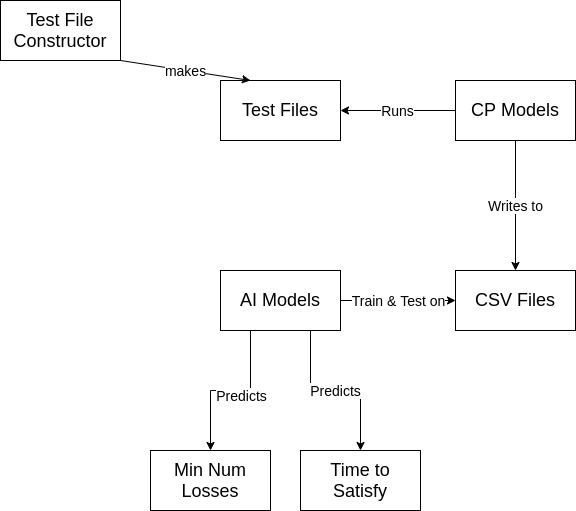
\includegraphics[width=\textwidth]{fyp_outline}
		\caption{Diagram of System Implementation}
	\end{figure}
	
	\newpage
	\section{Implementation}
	
	\subsection{Constraint Program Model}
	Minizinc and Gecode were used to run the constraint problems. Minizinc is a free and open-source constraint modelling language. Gecode is an open source C++ toolkit for developing constraint-based systems and applications.  To extract features from the test dataset, a feature extractor tool was needed. As a result, the program 'mzn2feat' was chosen to extract an extensive 95 features from each Constraint Satisfaction Problem and stored into a CSV file along with the number of constraints, number of fixtures left, number of teams, and the runtime of the sample.  
	
	\subsection{Machine Learning Models}
	For AI development, Python with Jupyter Notebook were used due to familiarity, simplicity, and it’s visualisation features. The Python libraries ‘pandas’, ‘numpy’, and ‘sklearn’ made it very easy to develop different types of AI models to test on the datasets. Pandas is an open source data analysis and manipulation tool, Numpy is a python package for scientific computing, and Sklearn is a machine learning library.
	Once enough information was gathered from the test sets, machine learning models were developed to predict two values. The runtime of an algorithm on a given problem, and the minimum number of losses problem [reference to where this was explained]. Machine Learning (ML) is the scientific study of algorithms and statistical models that computer systems use to perform a specific task without using explicit instructions, relying on patterns and inference instead. In this paper, we investigate the accuracy of three different ML models on our problem set. Linear Regression, Random Forest, and Decision Trees. These models were chosen as they use different learning methods.
	
	Linear Regression: Linear regression is a machine learning algorithm based on supervised learning. Reinforcement learning is an area of machine learning concerned with how software agents ought to take actions in an environment in order to maximize the notion of cumulative reward.
	
	Decision Trees: Decision tree learning is one of the predictive modeling approaches used in  machine learning. It uses a decision tree (as a predictive model) to go from observations about an item (represented in the branches) to conclusions about the item's target value (represented in the leaves). Decision trees where the target variable can take continuous values (typically real numbers) are called regression trees.
	
	Random Forest: Random forests or random decision forests are an ensemble learning method for classification, regression and other tasks that operate by constructing a multitude of decision trees at training time and outputting the class that is the mode of the classes (classification) or mean prediction (regression) of the individual trees.[1][2]
	
	\subsection{Test Evaluation}
	The test set was ran using a python script from terminal on up to 20,000 test sets. The machine that this was run on was a Dell Inspiron 13 5000 Series-5390. This computer uses 8GB RAM with a 8 x Intel® Core™ i7-8565U CPU @ 1.80GHz processor. Ubuntu 18.04.3 LTS was the operating system used. Each test was run with a 15 second maximum running time. Due to the dramatic increase of complexity of constraint programming problems, an upper bound of time was a necessity. 
	
	Test sets differed by the introduction of three variables. Number of teams, fixtures left, and number of constraints. The number of teams was the quantity of teams that were participating in the competition. Fixtures left was a parameter that defined how many fixtures were left until the end of the competition. Number of constraints defined how many positional constraints the test set was using. The remaining games have been previously simulated [refer back to where this was described] and therefore have a guaranteed satisfiable result. The tests were then recorded and stored by writing a script which utilises the python libraries ‘os’ and ‘csv’. The library os provides a portable way of using operating system dependent functionality [reference]. Using this library allowed for quick navigation through the test directories in order to run the problems. The csv library implements classes to read and write tabular data in CSV format [reference]. The library was used to record each test result into a CSV file.
	
	Below, is an example of a test set being generated, with 6 teams. This example is taken from the file located in LeagueTestMiniZinc6Teams/1GamesLeft/1Constraint:
	
	\begin{table}[h!]
		\centering
		\begin{tabular}{ |p{3cm}||p{3cm}| |p{3cm}| }
			\hline\multicolumn{3}{|c|}{6 Team League Example} \\
			\hline
			\hline
			Team Number & Games Played (Out of 10) & Points in Competition\\
			\hline
			1   & 10    & 4\\
			2&   10  & 17\\
			3 & 9 & 14\\
			4 & 8 & 15\\
			5&   9  & 15\\
			6& 8  & 11\\
			\hline
		\end{tabular}
		\caption{An example of a competition problem instance.}
	\end{table}
	
	For training the AI models to predict runtime, examples that ran over the designated time limit were removed from the dataset. The reason for this the resulting time limit was not a true reflection of how long the constraint model spent to generate a solution. In reality, these solutions would have taken much longer. A similar technique was used for predicting the minimum number of losses problem [reference]. Values that didn’t find a solution within the 15 second time limit were assigned a value of -1. Because this is not a valid solution, these examples were removed.
	
	Each AI model must be compared and evaluated against one another to determine which one is most accurate. There are various methods to measure this. The method used in this paper is Root Mean Squared Error (RMSE):
	
	
	\(\vect{m}\): The number of examples in the dataset
	
	\(\vect{h}_{\vect{\beta}}\): The model to be tested
	
	\(\vect{x}^{(i)}\): The input values of example \(i\)
	
	\(\vect{y}^{(i)}\): The actual result for example \(i\)
	
	\(\vect{h}_{\vect{\beta}}(\vect{x}^{(i)})\): The estimated prediction of \(\vect{x}^{(i)}\) using model 	\(\vect{h}_{\vect{\beta}}\)
	
	\begin{equation}
		\sqrt{\frac{1}{m} \sum_{i=1}^{\vect{m}} (\vect{h}_{\vect{\beta}}(\vect{x}^{(i)}) - \vect{y}^{(i)})^2}
	\end{equation}
	The reason for using this estimator over e.g. Mean Absolute Error (MAE) is because it penalises models that are accurate but estimate occasional wildly inaccurate results. 
	
	
	
	\subsection{Challenges}
	Challenges
	When creating the constraint model for minimising the number of losses, the initial implementation had it stored in a n x n matrix, where n was the number of teams in the league. However, it was later realised that a much more optimal solution was to create an n x m matrix, where m was the number of fixtures left in the league. This is because we do not need to store every loss occurring against every team, only the remaining games. The resulting model greatly increased efficiency. 
	
	I encountered a model inconsistency error for a prolonged period of time when developing the minimum number of losses constraint model. A model inconsistency error occurs when the program that translates the Minizinc file detects that the model is unsolvable. After some time, I realised the \(num\_losses\) variable was not 0 inclusive, which it needed to be. By redefining the variable to be 0 inclusive resolved the issue.
	
	Making the AI models was not very problem inducing. The construction and running of the programs did not create much complications. However, the performance of the models on the test set were incredibly inaccurate. This was due to the 15 second time limit on the programs. Many of the problems with high complexity ran up to 15 seconds. As a result, many of the models consistently guessed 15 for every problem. To combat this, all 15 second timeout problems were removed from the training set so as not to contaminate the model. This change made a dramatic improvement on the model.
	Another problem with the 15 second timeout values, is that they would not have a minimum number of losses value, as they did not return a solution. To fix this, a default value of -1 was imputed to imply that it was not terminated. As a result, these models discarded the sets with a -1 value.
	
	

	\newpage
	\section{Evaluation}
	
	\subsection{Tables}
	
	\begin{table}[h!]
		\centering
		\begin{tabular}{ |p{1.5cm}||p{3cm}| |p{3cm}| }
			\hline\multicolumn{3}{|c|}{Average Runtime (s) for Number of Fixtures Left in the League} \\
			\hline
			\hline
			Fixtures Left & Satisfiability & Minimum Number of Losses\\
			\hline
			1   & 0.0648    & 0.0691\\
			2&   0.0657  & 0.1460\\
			3 & 0.1146 & 0.6035\\
			4 & 0.3649 & 1.3468\\
			5&   1.5640  & 3.4737\\
			6& 2.4187  & 4.8700\\
			7& 4.2685  & 6.7400\\
			8& 5.2177  & 8.1034\\
			9& 6.4027  & 8.6409\\
			10& 6.8905  & 9.4665\\
			11& 6.3793  & 9.3531\\
			12& 7.2798  & 9.3114\\
			13& 8.2878  & 10.0541\\
			14& 7.5425  & 10.4122\\
			15& 9.2445  & 12.2531\\
			16& 8.2650  & 12.3536\\
			\hline
		\end{tabular}
		\caption{Average runtime of the Satisfiability problem, and the Minimum Number of Losses problem, in respect to a change in number of fixtures remaining in the competition.}
	\end{table}
	
	\begin{table}
		\centering
		\begin{tabular}{ |p{1.5cm}||p{3cm}| |p{3cm}| }
			\hline\multicolumn{3}{|c|}{Average Runtime (s) for Number of Positional Constraints} \\
			\hline
			\hline
			Number of Constraints & Satisfiability & Minimum Number of Losses\\
			\hline
			1   & 1.0996    & 1.6571\\
			2&   1.9524  & 2.9934\\
			3 & 2.5539 & 3.7771\\
			4 & 3.2378 & 4.8580\\
			5&   3.8842  & 5.2777\\
			\hline
		\end{tabular}
		\caption{Average runtime of the Satisfiability problem, and the Minimum Number of Losses problem, in respect to a change in number of positional constraints.}
	\end{table}

	\begin{table}
		\centering
		\begin{tabular}{ |p{1.5cm}||p{3cm}| |p{3cm}| }
			\hline\multicolumn{3}{|c|}{Average Runtime (s) for Number of Teams} \\
			\hline
			\hline
			Number of Teams & Satisfiability & Minimum Number of Losses \\
			\hline
			6   & 0.0310    & 0.0426\\
			7&   0.0401  & 0.5032\\
			8 & 0.1937 & 1.0445\\
			9 & 1.0982 & 1.8692\\
			10&   1.4043  & 2.3744\\
			11&   2.3964  & 3.9791\\
			12&   2.4323  & 4.0073\\
			13&   2.7928  & 4.9153\\
			14&   3.5149  & 6.0994\\
			15&   4.1257  & 6.3476\\
			16&   4.5801  & 6.0267\\
			17&   4.7206  & 6.8090\\
			18&   5.4237  & 7.3615\\
			\hline
		\end{tabular}
		\caption{Average runtime of the Satisfiability problem, and the Minimum Number of Losses problem, in respect to a change in number of teams in the competition.}
	\end{table}

	\begin{figure}
		\centering
		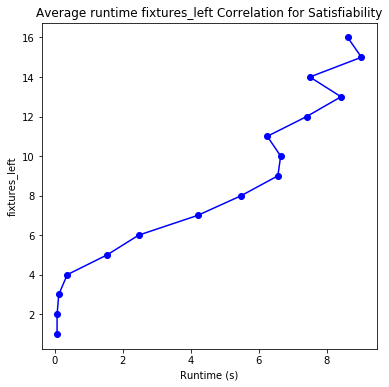
\includegraphics[width=0.7\linewidth]{graphs/LR/rt-fix_left-LR}
		\caption{The average runtime of the satisfiability problem set in respect to the number of fixtures left in the competition.}
		\label{fig:rt-fixleft-lr}
	\end{figure}
	\begin{figure}
		\centering
		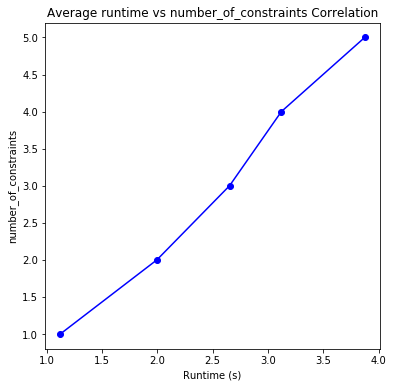
\includegraphics[width=0.7\linewidth]{graphs/LR/rt-num_const-LR}
		\caption{The average runtime of the satisfiability problems in respect to the number of suppositions within the problem.}
		\label{fig:rt-numconst-lr}
	\end{figure}
	\begin{figure}
		\centering
		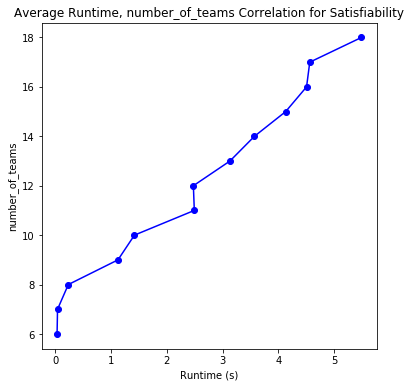
\includegraphics[width=0.7\linewidth]{graphs/LR/rt-num_teams-LR}
		\caption{The average runtime of the satisfiability problems in respect to the number of teams in the problem set.}
		\label{fig:rt-numteam-lr}
	\end{figure}
	\begin{figure}
		\centering
		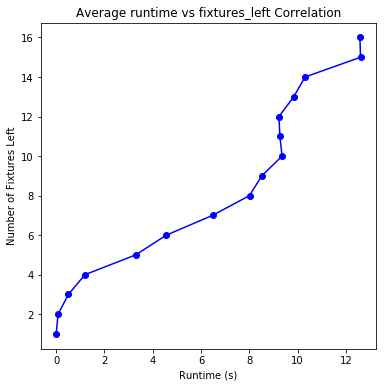
\includegraphics[width=0.7\linewidth]{graphs/LR/mnl-fix_left-LR}
		\caption{The average runtime of the minimum number of losses problem set in respect to the number of fixtures left in the competition.}
		\label{fig:mnl-fix_left-lr}
	\end{figure}
	\begin{figure}
		\centering
		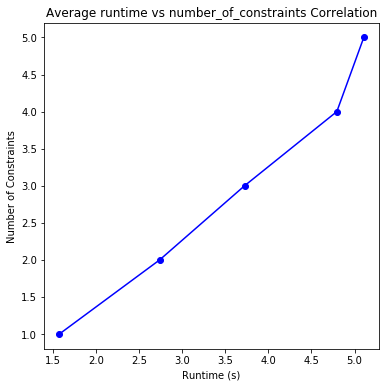
\includegraphics[width=0.7\linewidth]{graphs/LR/mnl-num_const-LR}
		\caption{The average runtime of the minimum number of losses problems in respect to the number of suppositions within the problem.}
		\label{fig:mnl-num_const-lr}
	\end{figure}
	\begin{figure}
		\centering
		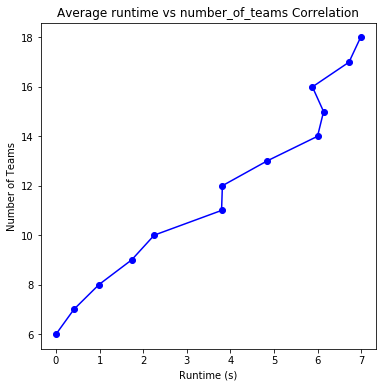
\includegraphics[width=0.7\linewidth]{graphs/LR/mnl-num_teams_LR}
		\caption{The average runtime of the minimum number of losses problems in respect to the number of teams in the problem set.}
		\label{fig:mnl-num_teams_lr}
	\end{figure}

	\begin{figure}
		\centering
		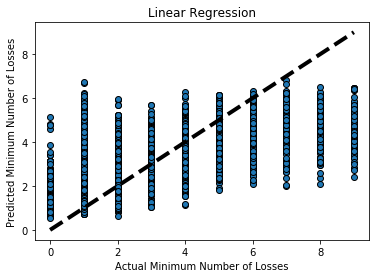
\includegraphics[width=0.7\linewidth]{graphs/LR/est-act-predict-LR-mnl}
		\caption{Estimated vs Actual predictions for the minimum number of losses problem using Linear Regression}
		\label{fig:est-act-predict-mnl}
	\end{figure}
	\begin{figure}
		\centering
		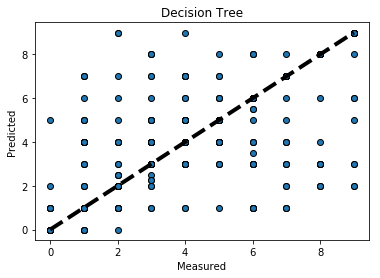
\includegraphics[width=0.7\linewidth]{graphs/DT/est-act-predict-DT-mnl}
		\caption{Estimated vs Actual predictions for the minimum number of losses problem using Decision Trees}
		\label{fig:est-act-predict-dt}
	\end{figure}
	\begin{figure}
		\centering
		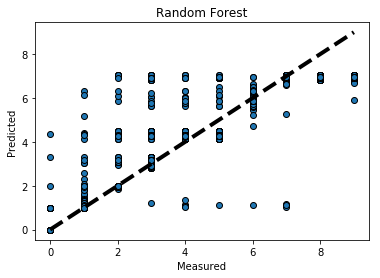
\includegraphics[width=0.7\linewidth]{graphs/RF/est-act-predict-RF-mnl}
		\caption{Estimated vs Actual predictions for the minimum number of losses problem using Random Forest}
		\label{fig:est-act-predict-rf}
	\end{figure}
	\begin{figure}
		\centering
		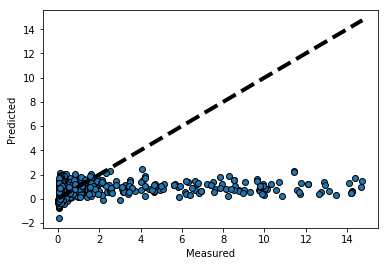
\includegraphics[width=0.7\linewidth]{graphs/LR/est-act-predict-LR-sat}
		\caption{Estimated vs Actual predictions for runtime satisfiability using Linear Regression}
		\label{fig:est-act-predict-mnl-sat}
	\end{figure}
	\begin{figure}
		\centering
		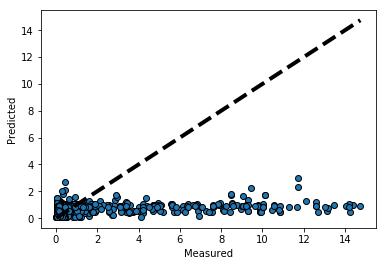
\includegraphics[width=0.7\linewidth]{graphs/RF/est-act-predict-RF-sat}
		\caption{Estimated vs Actual predictions for runtime satisfiability using Random Forest}
		\label{fig:est-act-predict-rf-sat}
	\end{figure}
	\begin{figure}
		\centering
		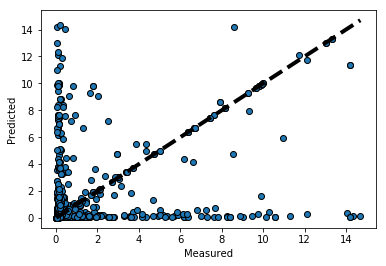
\includegraphics[width=0.7\linewidth]{graphs/DT/est-act-predict-DT-sat}
		\caption{Estimated vs Actual predictions for runtime satisfiability problem using Decision Trees}
		\label{fig:est-act-predict-dt-sat}
	\end{figure}


	\begin{table}[h!]
		\centering
		\begin{tabular}{ |p{3cm}||p{1.5cm}| |p{1.5cm}| }
			\hline\multicolumn{3}{|c|}{Root Mean Squared Error (RMSE) for AI Models} \\
			\hline
			\hline
			Model Type & Runtime & Minimum Number of Losses\\
			\hline
			Linear Regression   & -1.9712    & -3.3310\\
			Random Forest &   -1.8338  & -0.5283\\
			Decision Tree & -1.9254 & -0.4703\\
			\hline
		\end{tabular}
		\caption{Negative mean squared error values for predicting the Runtime of the Satisfiability problem, and the minimum number of losses in the Minimum Number of Losses Problem.}
	\end{table}

	\begin{table}
		\centering
		\begin{tabular}{ |p{3cm}||p{3cm}| |p{3cm}| }
			\hline\multicolumn{3}{|c|}{Correlation Coefficient of AI Models} \\
			\hline
			\hline
			Model Type & Runtime Prediction & Minimum Number of Losses Prediction\\
			\hline
			Linear Regression   & 0.2727    & 0.6281\\
			Random Forest &   0.2895  & 0.9531\\
			Decision Tree & 0.5113 & 0.9579\\
			\hline
		\end{tabular}
		\caption{Correlation Coefficienct for predicting the Runtime of the Satisfiability problem, and the minimum number of losses in the Minimum Number of Losses Problem.}
	\end{table}




	
	\newpage
	\section{Conclusions}
	It’s clear to see from the tables, that an increase in fixtures, teams, or constraints will lead to an increase in runtime. This is due to the increase in complexity of the problem. The rate of increase seems to occur exponentially for the case of fixtures left, but not as dramatic for number of constraints, or number of teams. The Satisfiability constraint model was much faster than the Minimum Number of Losses Optimisation model. This was expected due to the SAT model only needing to find the first solution it finds within the search space. The optimisation problem proves much more difficult as the search tree must be traversed through many possible solutions, before returning with an optimal solution. 
	
	
	\newpage

	\begin{thebibliography}{9}
		\bibitem{threepointrule}
		T. Bernholt, A. G¨alich, T. Hofmeister and N. Schmitt, Football elimination is hard to decide
		under the 3-point-rule, International Symposium on Mathematical Foundations of Computer
		Science, (1999), 410–418.
		\bibitem{cp}
		Barbara M. Smith: A Tutorial on Constraint Programming, TR 95.14, University of Leeds,1995
		\bibitem{fifarules}
		 W. Kern and D. Paulusma, The new FIFA rules are hard: Complexity aspects of sports competitions, Discrete Applied Mathematics, 108 (2001), 317–323.
		\bibitem{eliminationproblem}
		W. Kern and D. Paulusma, The computational complexity of the elimination problem in generalized sports competitions, Discrete Optimization, 1 (2004), 205–214.
	\end{thebibliography}
	
	


\end{document}